Die Mathematik. Unendliche Weiten. Dieses sind die Abenteuer einiger
Studenten, die sich auf einer Dreijahresmission in den Tiefen der Räume und
Gruppen befinden, um während ihrer Reise auf der USS Prüfungsordnung neue Sätze
und Formeln zu erforschen. Leider ist der Kontakt zur Mutterzivilisation auf
der Erde längst abgebrochen.

So oder so ähnlich würde die Einleitung einer Fernsehserie zum Studium der
Mathematik wohl lauten. Aber wir sind hier ja nicht im Fernsehen. Und trotzdem
-- oder vielleicht auch gerade deswegen -- klingt es erschreckend realistisch.
Nach allgemeiner Meinung schwebt die Mathematik mehr als jede andere
Wissenschaft im luftleeren Raum. Mathematiker werden im wahren Sinne des Wortes
als weltfremd erachtet. Die Mathematik wird häufig mit Analoga umschrieben:
Mathe sei Kunst, Religion, Sprache, Philosophie, die reinste aller
Wissenschaften. Und doch weiß praktisch niemand, was Mathematik wirklich ist.
Vielleicht ist der Kontakt von der Erde ja absichtlich abgebrochen worden?

Wenn man rein berufsorientiert argumentieren will, kann man sagen, dass
Mathematik eine Daseinsberechtigung haben muss, sonst würden Mathematiker nicht
eingestellt werden. Aber welche? Und wie steht es mit der Mathematik und ihren
Anwendungen außerhalb des \emph{echten} Berufslebens? Ist die Mathematik nur
eine Hilfswissenschaft für Physik, Sozial-, Ingenieur- und
Wirtschaftswissenschaften, oder hat sie einen Wert an sich, als \emph{L'art
pour l'art} gewissermaßen?

In der Einheit Mathematik und Gesellschaft am Mittwoch, 12.10. wollen wir uns
mit dieser Problematik auseinander setzen. Was ist Mathematik eigentlich? Was
ist Mathematik nicht? Wie stehen die Mathematik und die Mathematiker in der
Gesellschaft? Tun sie das überhaupt? Wie steht die Gesellschaft zur Mathematik
und zu den Mathematikern? Was kann der Mathematiker von der Gesellschaft
verlangen, was kann, soll und muss er ihr zurückgeben? Und inwiefern ist der
Mathematiker für seine Forschung und deren Wirkungen in die Gesellschaft hinein
verantwortlich?

Selbstverständlich können wir in der kurzen Zeit dieses Thema nicht annähernd
vollständig behandeln -- aber wir werden versuchen, euch Anregungen zu geben.
Wir werden euch mit Fragen konfrontieren, die nicht unbedingt eine Antwort
haben, die man aber trotzdem stellen sollte -- ganz entgegen der landläufigen
Meinung zum Thema Mathematik, die ja auf alle Fragen eindeutige Lösungen kennen
soll (wohlgemerkt: die Mathematik; der Mathematiker kennt sie oft noch nicht).
Außerdem wollen wir aufdecken, wie die Mathematik benutzt oder gar missbraucht
wird, um Objektivität und Sicherheit vorzutäuschen -- dieses Versprechen aber,
wieder entgegen aller Vorurteile, bei weitem nicht immer halten kann.

\begin{center}
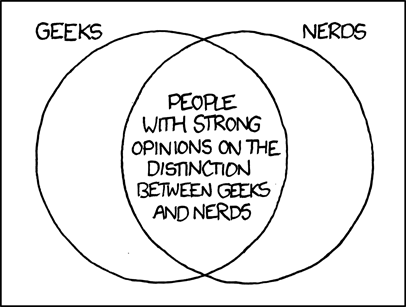
\includegraphics[scale=0.75]{comics/747}
\end{center}

Lange Zeit hat sich die Mathematik weniger um ihre gesellschaftlichen
Verpflichtungen, Berührungspunkte und Zusammenhänge, sondern mehr um sich
selbst gekümmert. Dadurch haben viele Mathematiker die Verwendung ihrer
Arbeiten und den Umgang mit Mathematik in der Gesellschaft und auch in den
anderen Wissenschaften aus den Augen verloren. Unser Wunsch ist es, euch zu
weiterem Nachdenken anzuregen und dass ihr euch mit diesen Fragen
auseinandersetzt, weil es zu verstehen hilft, warum ihr gerade Mathematik
studiert. 

Und weil es hilft, den Kontakt zur Erde vielleicht doch noch aufrecht zu
erhalten.
